%% Le lingue utilizzate, che verranno passate come opzioni al pacchetto babel. Come sempre, l'ultima indicata sar� quella primaria.
%% Se si utilizzano una o pi� lingue diverse da "italian" o "english", leggere le istruzioni in fondo.
\def\thudbabelopt{english}
%% Valori ammessi per target: bach (tesi triennale), mst (tesi magistrale), phd (tesi di dottorato).
\documentclass[target=bach]{thud}[2014/03/11]
\usepackage{adjustbox}
\usepackage{tabularx}
\usepackage{float}
\usepackage{hyperref}
\usepackage{graphicx}
%\usepackage{bera}% optional: just to have a nice mono-spaced font
\usepackage{listings}
\usepackage{xcolor}
%\usepackage{natbib}
\usepackage{tocbibind}
\usepackage{mathtools}

\definecolor{lightgray}{rgb}{0.95, 0.95, 0.95}
\definecolor{darkgray}{rgb}{0.4, 0.4, 0.4}
%\definecolor{purple}{rgb}{0.65, 0.12, 0.82}
\definecolor{editorGray}{rgb}{0.95, 0.95, 0.95}
\definecolor{editorOcher}{rgb}{1, 0.5, 0} % #FF7F00 -> rgb(239, 169, 0)
\definecolor{editorGreen}{rgb}{0, 0.5, 0} % #007C00 -> rgb(0, 124, 0)
\definecolor{orange}{rgb}{1,0.45,0.13}		
\definecolor{olive}{rgb}{0.17,0.59,0.20}
\definecolor{brown}{rgb}{0.69,0.31,0.31}
\definecolor{purple}{rgb}{0.38,0.18,0.81}
\definecolor{lightblue}{rgb}{0.1,0.57,0.7}
\definecolor{lightred}{rgb}{1,0.4,0.5}

\lstdefinelanguage{JavaScript}{
  morekeywords={typeof, new, true, false, catch, function, return, null, catch, switch, var, if, in, while, do, else, case, break},
  morecomment=[s]{/*}{*/},
  morecomment=[l]//,
  frame=lines,
  morestring=[b]",
  morestring=[b]'
}

\colorlet{punct}{red!60!black}
\definecolor{background}{HTML}{EEEEEE}
\definecolor{delim}{RGB}{20,105,176}
\colorlet{numb}{magenta!60!black}
\definecolor{color:keyword}{rgb}{0.53,0.05,0.05}
\definecolor{color:comment}{rgb}{0.25,0.37,0.75}
\definecolor{color:string}{rgb}{0.87,0.0,0.0}

\lstdefinelanguage{Jolie}{
 morekeywords={csets,type,raw,any,undefined,void,default,if,for,while,spawn,foreach,else,define,main,include,constants,inputPort,outputPort,interface,execution,cset,nullProcess,RequestResponse,OneWay,throw,throws,install,scope,embedded,init,synchronized,global,is_defined,is_int,is_bool,is_long,is_string,bool,long,int,string,double,undef,with,Location,Protocol,Interfaces,Aggregates,Redirects,linkIn,linkOut},
 sensitive=true,
 morecomment=[l]{//},
 morecomment=[s]{/*}{*/},
 morestring=[b]",
 otherkeywords={;,|,@}
}

\lstset{
 language=Jolie,
 mathescape=true,
 resetmargins=true,
 numberstyle=\footnotesize,
 numbers=left,
 numbersep=5pt,
 numberblanklines=true,
 basicstyle=\ttfamily\small,
 tabsize=2,
 frame=lines,
 commentstyle=\ttfamily\color{color:comment},
 stringstyle=\color{color:string},
 captionpos=b,
 keywordstyle=\bfseries\color{color:keyword},
 showstringspaces=false,
 belowcaptionskip=10mm,
 breaklines=false,
 columns=fullflexible,
 linewidth= 0.8\linewidth
}


\colorlet{punct}{red!60!black}
\definecolor{keyword}{RGB}{48,0,211}
\colorlet{numb}{magenta!60!black}

\newcommand{\kwd}[1]{{\color{keyword}\textbf{#1}}}
\newcommand{\hid}[1]{{\color{gray}#1}}

\lstdefinelanguage{json}{
    basicstyle=\ttfamily\small,
    commentstyle=\color{color:comment}, % style of comment
    stringstyle=\color{color:string}, % style of strings
    numbers=left,
    numberstyle=\scriptsize,
    stepnumber=1,
    numbersep=8pt,
    showstringspaces=false,
    frame=lines,
    string=[s]{"}{"},
    comment=[l]{:\ "},
    morecomment=[l]{:"},
    literate=
        *{0}{{{\color{numb}0}}}{1}
         {1}{{{\color{numb}1}}}{1}
         {2}{{{\color{numb}2}}}{1}
         {3}{{{\color{numb}3}}}{1}
         {4}{{{\color{numb}4}}}{1}
         {5}{{{\color{numb}5}}}{1}
         {6}{{{\color{numb}6}}}{1}
         {7}{{{\color{numb}7}}}{1}
         {8}{{{\color{numb}8}}}{1}
         {9}{{{\color{numb}9}}}{1}
         {\$}{{{\color{numb}{\$}}}}{1}
}
%\lstdefinelanguage{json}{
%    basicstyle=\normalfont\ttfamily,
%    numbers=left,
%    numberstyle=\scriptsize,
%    stepnumber=1,
%    numbersep=8pt,
%    showstringspaces=false,
%    breaklines=true,
%    frame=lines,
%    backgroundcolor=\color{background},
%    literate=
%     *{0}{{{\color{numb}0}}}{1}
%      {1}{{{\color{numb}1}}}{1}
%      {2}{{{\color{numb}2}}}{1}
%      {3}{{{\color{numb}3}}}{1}
%      {4}{{{\color{numb}4}}}{1}
%      {5}{{{\color{numb}5}}}{1}
%      {6}{{{\color{numb}6}}}{1}
%      {7}{{{\color{numb}7}}}{1}
%      {8}{{{\color{numb}8}}}{1}
%      {9}{{{\color{numb}9}}}{1}
%      {:}{{{\color{punct}{:}}}}{1}
%      {,}{{{\color{punct}{,}}}}{1}
%      {\{}{{{\color{delim}{\{}}}}{1}
%      {\}}{{{\color{delim}{\}}}}}{1}
%      {[}{{{\color{delim}{[}}}}{1}
%      {]}{{{\color{delim}{]}}}}{1},
%}


%% --- Informazioni sulla tesi ---
%% Per tutti i tipi di tesi
\title{Design and implementation of a Language Server for the Jolie programming language}
\author{Eros Fabrici}
\course{Tecnologie Web e Multimediali}
\supervisor{Prof.\ Marino Miculan}
%% Altri campi disponibili: \reviewer, \tutor, \chair, \date (anno accademico, calcolato in automatico).
%% Con \supervisor, \cosupervisor, \reviewer e \tutor si possono indicare pi� nomi separati da \and.
%% Per le sole tesi di dottorato
%%\phdnumber{313}
%%\cycle{XXVIII}
%%\contacts{Via della Sintassi Astratta, 0/1\\65536 Gigatera --- Italia\\+39 0123 456789\\\texttt{http://www.example.com}\\\texttt{inbox@example.com}}
%%\rights{Tutti i diritti riservati a me stesso e basta.}
%% Campi obbligatori: \title, \author e \course.

%% --- Pacchetti consigliati ---
%% hyperref: Regola le impostazioni della creazione del PDF... pi� tante altre cose.
%% tocbibind: Inserisce nell'indice anche la lista delle figure, la bibliografia, ecc.

%% --- Stili di pagina disponibili (comando \pagestyle) ---
%% sfbig (predefinito): Apertura delle parti e dei capitoli col numero grande; titoli delle parti e dei capitoli e intestazioni di pagina in sans serif.
%% big: Come "sfbig", solo serif.
%% plain: Apertura delle parti e dei capitoli tradizionali di LaTeX; intestazioni di pagina come "big".

\begin{document}

%% Il frontespizio prima di tutto!
\maketitle

%% Dedica (opzionale)
\begin{dedication}Al mio cane,\par per avermi ascoltato mentre ripassavo le lezioni.\end{dedication}

%% Ringraziamenti (opzionali)
\acknowledgements
Sed vel lorem a arcu faucibus aliquet eu semper tortor. Aliquam dolor lacus, semper vitae ligula sed, blandit iaculis leo. Nam pharetra lobortis leo nec auctor. Pellentesque habitant morbi tristique senectus et netus et malesuada fames ac turpis egestas. Fusce ac risus pulvinar, congue eros non, interdum metus. Mauris tincidunt neque et aliquam imperdiet. Aenean ac tellus id nibh pellentesque pulvinar ut eu lacus. Proin tempor facilisis tortor, et hendrerit purus commodo laoreet. Quisque sed augue id ligula consectetur adipiscing. Vestibulum libero metus, lacinia ac vestibulum eu, varius non arcu. Nam et gravida velit.

%% Sommario (opzionale)
\abstract
Nunc ac dignissim ipsum, quis pulvinar elit. Mauris congue nec leo ornare lobortis. Nulla hendrerit pretium diam nec lobortis. Nullam aliquam laoreet nisl, sit amet facilisis lectus accumsan ut. Duis et elit hendrerit metus venenatis condimentum. Integer id eros molestie, interdum leo sit amet, aliquet metus. Integer fermentum tristique magna, vel luctus neque rhoncus vel. Ut hendrerit et quam et semper. Mauris egestas, odio sed aliquet luctus, magna orci euismod odio, vitae lacinia tellus tellus non lectus. Aliquam urna neque, porta et mattis aliquam, congue sit amet lorem. In ultrices augue sit amet ante vehicula, vitae rhoncus turpis auctor. Donec porta scelerisque eros, at mollis enim imperdiet ut. 

%% Indice
\tableofcontents

%% Lista delle tabelle (se presenti)
%\listoftables

%% Lista delle figure (se presenti)
%\listoffigures

%% Corpo principale del documento
\mainmatter

%% Parte
%% La suddivisione in parti � opzionale; talvolta sono sufficienti i capitoli.

%% Capitolo
\chapter{Introduction}
%%Problem: implementing advance IDE functionalities for the Jolie language to be added in Microsoft Vs-code and similar

\chapter{Jolie and the Language Server Protocol}
\label{sec:JolieLSP}
\section{Jolie: Java Orchestration Language Interpreter Engine}
Service-Oriented Computing (SOC) is a design methodology that focuses on the
composition of autonomous entities in a system, called services. SOC abstracts
from the implementation details of services by imposing a standard communication mechanism between the entities in an SOA (Service-Oriented Architecture)\cite{Jol}. From the perspective the aforementioned methodologies, it is possible to identify a separation between \textit{behavioral} and \textit{architectural} composition of services. The first denotes a series of interactions to be performed in order to reach a goal, while the second deals with the topological structure of a SOA, managing its execution and integration. The lack of an homogeneous solution between the \textit{behavioral} and the \textit{architectural} composition of services require ad-hoc interventions in order to integrate them, which will make the entire architecture less modular and difficult to maintain.\\\textbf{Jolie} was created with the intention to fill the aforementioned gap. This language permits to define services, their behavioral composition, supporting different communication technologies, and their organization inside a SOA.
\subsection{Language basics: behavior and deployment}
A Jolie program defines a service, which is composed by two parts: the \textit{behavior} and the \textit{deployment}. The first defines the functionalities of the service, including primitives like communication and computation constructs. These does not define \textit{how} the communication is supported, they abstractly refer to \textit{communication ports} which are assumed to be correctly defined in the deployment part. For example, a behavioral primitive may express the action "ask the bank to show the actual balance", without knowing how to reach the "bank" service and which communication protocol it uses. These last two are handled by the deployment, which permits to define the \textit{location} and the \textit{protocol} of the bank service. Furthermore, the deployment permits the usage of architectural primitives for defining the architecture of a SOA. The syntax of a Jolie program is defined as the following:
\[Program \quad \Coloneqq \quad	D \quad \textcolor{color:keyword}{main}\,\{\, B\, \}\]
where D is the Deployment and B is the Behaviour. The \textcolor{color:keyword}{main} procedure is the execution entry point. 
\subsubsection{Behaviour}
Jolie syntax is a combination of the message passing and the imperative programming styles. 
Following a selection of the Jolie behavioral syntax:\\

{\setstretch{0.4}
\begin{align*}
	B \quad \Coloneqq&\, \eta \quad (input)\\
	|& \, \bar{\eta} \quad (output)\\
	|& \, \textcolor{color:keyword}{if}(e) \> B_1 \> \big[else \> B_2\big] \quad (condition)\\
	|& \, \textcolor{color:keyword}{while}(e) \> B \quad (while)\\
	|& \, \textcolor{color:keyword}{for}(init,\,cond,\,incr)\> B \quad (forLoop)\\
	|& \, \textcolor{color:keyword}{for}(x \, in \, y)\> B \quad (arrayIteration)\\
	|& \, B_1 \, ; \, B_2 \quad (sequential)\\
	|& \, B_1 \, | \, B_2 \quad (parallel)\\
	|& \, \{\, B \,\} \quad (block)\\
	|& \, x\,=\,e \quad (assign)\\
	|& \, a\,->\,e \quad (alias)\\
	|& \, x \, << \, y \quad (deepCopy)\\
	|& \, \big[\,\eta_1\,\big]\>\{\,B_1\,\}\,...\, \big[\,\eta_n\,\big]\>\{\,B_n\,\} \quad (inputChoice)\\
	|& \, \textcolor{color:keyword}{scope}(s) \> \{\,B\,\} \quad (scope)\\
	|& \, \textcolor{color:keyword}{install}(\,h_1\> => \>B_1,...,\,h_n\> => \> B_n) \quad (install)\\
	|& \, \textcolor{color:keyword}{throw}(f[,\,x]) \quad (throw)
\end{align*}
%	|& \, \textcolor{color:keyword}{cH} \quad (cH)\\
where
\begin{align*}
	\eta \quad \Coloneqq&\, opName(x) \quad (OneWay)\\
	|& \, opName(x)(e)\>\{\,B\,\} \quad (RequestResponse)
\end{align*}\\
and
\begin{align*}
	\bar{\eta} \quad \Coloneqq&\, opName\textcolor{color:keyword}{@}OP(e) \quad (notification)\\
	|&\, opName\textcolor{color:keyword}{@}OP(e)(x) \quad (SolcitResponse)
\end{align*}
}
\textbf{Communications} are implemented through \textit{Rules} \textit{(input)}, \textit{(output)} and \textit{(inputChoice)}. Input $\boldsymbol\eta$ can be either a \textit{OneWay} or a \textit{RequestResponse}. The first receives a message for the operation \textit{opName} and saves its content in variable \verb|x|, while the second receives a message for operation \textit{opName} in variable \verb|x|, executes behavior \textit{B} and sends the value of the evaluation of the expression \textit{e} to the invoker. \textit{(notification)} and \textit{(SolcitResponse)}  implement the output towards the input . The first sends a message with the evaluation of \textit{e}, the second does the same thing and waits for the response from the invoked service which is stored in the var \verb|x|. \textit{OP} denotes the \textbf{output port name} that references an \textcolor{color:keyword}{outputPort}. The latter is specified in the deployment definition and it contains all the necessary information in order to contact the target service. Lastly, the \textit{(inputChoice)} supports the receiving of a message for any of the inputs. When a message for the input $\eta_i$ is received, all the remaining branches are deactivated and $\eta_i$ is executed. Afterwards, $B_i$ is executed. The interpreter enforces that $\eta_i \neq \eta_j,\,\forall i,j \in [1,n] \, | \, i \neq j$, which means that there cannot be two inputs with the same operation.\\\textbf{Statement compositions}, such that \textit{(condition)}, \textit{(while)}, \textit{(forLoop)}, \textit{(arrayIteration)} and \textit{(block)}, resembles the ones used in classic imperative styles. Rule \textit{sequential} sequentially compose the two behaviors: when $B_1$ is terminated, $B_2$ can start its execution (remark: the separator \textit{;} is now optional). On the contrary, \textit{(parallel)} permits the parallel execution of the two behaviors.\\\textbf{Assignment and aliasing}: \textit{(assign)} evaluates the expression \textit{e} and assigns its value to the variable \verb|x|. \textit{(alias)} permits to define a variable $a$ that points to $x$ variable path.\\\textbf{Handling data} Jolie is dynamically-typed meaning that there is no necessity of type declarations and that the type of a variable value is checked at runtime. The language handles the following basic data types:
\begin{itemize}
	\item \verb|bool|: booleans;
	\item \verb|int|: integers;	
	\item \verb|long|: long integers (with \verb|l| or \verb|L| suffix);
	\item \verb|double|: double-precision float;
	\item \verb|string|: strings;
	\item \verb|raw|: byte arrays (supported for data-passing purposes);
	\item \verb|void|: the empty type.
\end{itemize}
Jolie supports basic arithmetic and logic operators like in Java and also pre-/post-increment and pre-/post-decrement operators. Furthermore, it is possible to cast variables to other types with the following casting functions: \verb|bool()|, \verb|int()|, \verb|long()|, \verb|double()| and \verb|string()|. For instance:
\begin{lstlisting}[language=jolie]
	d = "1.5"
	n = double( d ) // n = 1.5
	n = int( n ) // n = 1
\end{lstlisting}
A variable type can be checked at runtype with the \textcolor{color:keyword}{instanceof} operator, whose syntax is:
\[expression \>\> \textcolor{color:keyword}{instanceof} \>\> (native\_type\,|\,custom\_type)\]
Variables are undefined until they are assigned a value. Until then, their state is set to \textcolor{color:keyword}{undefined} (equivalent to \verb|NULL|, \verb|null| or \verb|nil| in other languages). The predicate \textcolor{color:keyword}{is\_defined} is used for checking is a variable is defined or not. Following the syntax:
\[ \textcolor{color:keyword}{is\_defined} (\, variable\_name \,)\]
An example:
\begin{lstlisting}[language=jolie]
	x = 2
	if ( is_defined( x ) ) {
		println@Console( "Variable x is defined" )
	}
\end{lstlisting}
Arrays in Jolie are handled dynamically and can be accessed using the \verb|[]| operator. To be more precise, in Jolie \textbf{every} variable is a dynamic array. So for example this assignment
\begin{lstlisting}[language=jolie]
	x = 7
\end{lstlisting}
is equivalent to the following
\begin{lstlisting}[language=jolie]
	x[0] = 7
\end{lstlisting}
thus managing complex data is easier. To compute the size of an array Jolie provides the size operator \verb|#|. Together with this operator, the aforementioned \textit{forLoop} can be used to traverse an array. Alternatively, \textit{(arrayIteration)} has the same purpose. The example below shows the usage of the mentioned constructs.
\begin{lstlisting}[language=jolie]
	x[0] = 1
	x[1] = 2
	x[2] = 3
	println@Console( #x )() // prints 3
	
	for( i = 0, i < #x, i++) {
		println@Console( x[i] )()	
	}
	//which is equivalent to
	for( el in x ) {
		println@Console( el )()	
	}
\end{lstlisting}
\textbf{Data structures} in Jolie are tree-like, similarly to XML or JSON data trees. The operator \verb|.| is used to traverse a data structure. Following an example.
\begin{lstlisting}[language=jolie]
	doctor.name = "Marco"
	doctor.surname = "Rossi"
	doctor.age = 45
	doctor.specialization[0] = "Cardiology"
	doctor.specialization[1] = "General Surgery"
\end{lstlisting}
The above data tree is catheterized by \verb|doctor| as root with \verb|void| type and by three children: \verb|name|, \verb|surname| and \verb|specialization| which respectively have the types \verb|string|, \verb|string|, \verb|int| and \verb|string|. The \textcolor{color:keyword}{undef} operator is used to erase an entire structure. Syntax:
\[\textcolor{color:keyword}{undef}(\,variable\_name\,) \]
The \textit{(deepCopy)} operator copies the entire structure of a tree $y$ into a tree $x$. Jolie at runtime explores the tree $y$ node-wise and for all initialised sub-nodes in $y$, it assigns the value of each of them to the corresponding sub-node rooted in $x$. This means that if $x$ already had sub-nodes initialised that correspondes to some ones rooted in $y$, $x \, << \, y$ will overwrite them, leaving all the others initialised nodes of $x$ unaffected. This operator can be used also as syntax sugar for creating a data structure. Basing on the previous example of the doctor data structure, in can be re-written in the following way.
\begin{lstlisting}[language=jolie]
	doctor << {
		name = "Marco"
		surname = "Rossi"
		birthDate << {
			day = 25
			month = 5
			year = 1971
		}
		specialization[0] = "Cardiology"
		specialization[1] = "General Surgery"
		email = "marco.rossi@gmail.com"
	}
\end{lstlisting}
\textbf{Fault handling:} Jolie has constructs to handle faults. The primitives meant for this purpose are: \textcolor{color:keyword}{scope}, \textcolor{color:keyword}{install} and \textcolor{color:keyword}{throw}. For more details see \cite{Jol}.
\subsubsection{Deployment}
The deployment is the part of a Jolie program in which all the necessary information for establishing communication channels between services are established. The basic primitives are \textit{input ports} and \textit{output ports} which are based on \textit{data types} and \textit{interfaces}. A deployment $D$ is simply a list of deployment instructions among which we can have input and output ports, type definitions, and interfaces \cite{Jol}:
%{\setstretch{0.4}
\begin{align*}
	D \>\> \Coloneqq& \>\> IP \quad (inputPort)\\
	|& \> OP \quad (outputPort)\\
	|& \> T_{def} \quad (typeDefinition)\\
	|& \> I \quad (interface)\\
	|& \> \textcolor{color:keyword}{execution}\{\, M \,\}\\
	|& \> E
\end{align*}
where 
\[ M \>\> \Coloneqq \>\> \textcolor{color:keyword}{single} \> | \> \textcolor{color:keyword}{sequential} \> | \> \textcolor{color:keyword}{concurrent} \]
\[ E \>\> \Coloneqq \>\> \textcolor{color:keyword}{embedded}\,\{\, E_{type}:\>path\,\big[\,\textcolor{color:keyword}{in} \> OP \, \big] \, \} \]
\[ E_{type} \>\> \Coloneqq \>\> \textcolor{color:keyword}{Jolie} \> | \> \textcolor{color:keyword}{Java} \> | \> \textcolor{color:keyword}{JavaScript} \]
%}
\textbf{Communication ports} are primitives that define \textit{how} communications with other services are handled. There are two kind of ports. $(inputPort)$ that exposes input operations to other services. Alternatively, $(outputPort)$ permits the invocation of other services' operations.\\The syntax for input and output port is the following.
%{\setstretch{0.4}
\begin{align*}
	IP \quad \Coloneqq \> &\textcolor{color:keyword}{inputPort}: \, id \> \{\\
	&\textcolor{color:keyword}{location}: \, URI\\
	&\textcolor{color:keyword}{protocol}: \, p\\
	&\textcolor{color:keyword}{interfaces}: \, I_1,\,I_2,...,\,I_n\\
	& \big[ \textcolor{color:keyword}{aggregates}: OP_1,...,OP_n\big]\\
	&\}
\end{align*}
\begin{align*}
	OP \quad \Coloneqq \> &\textcolor{color:keyword}{outputPort}: \, id \> \{\\
	&\textcolor{color:keyword}{location}: \, URI\\
	&\textcolor{color:keyword}{protocol}: \, p\\
	&\textcolor{color:keyword}{interfaces}: \, I_1,\,I_2,...,\,I_n\\
	&\}
\end{align*}
%}
These ports are based on three concepts of $location$, $protocol$ and $interface$. The former two define the concrete binding between the program and other services. In particular the $location$ must specify the communication medium. The mediums supported are: \textit{local} (jolie in-memory communication), \textit{socket}, \textit{btl2cap} (Bluetooth L2CAP), \textit{rmi} (Java RMI) and \textit{localsocket} (Unix local sockets). The $protocol$ indicates the data format. Jolie supports the following protocols: \textit{HTTP}, \textit{HTTPS}, \textit{JSON-RPC}, \textit{XML-RPC}, \textit{SOAP}, \textit{SODEP} (created and developed for Jolie), \textit{SODEPS} and \textit{RMI}. More details about the mediums and protocols can be found at \cite{JolieDoc}. The $interface$ defines a bind between the deployment and the behavior: more specifically it defines type information that is expected to be satisfied by the behavior that uses the ports.\\\textbf{Data types and interfaces}. Interfaces are a collection of operation types. The latter defines the type of the data to be communicated over each specified operation. Following the data type syntax.
\[ 
	T_{def} \>\> \Coloneqq \>\> \textcolor{color:keyword}{type} \> id \> T
\]

\[
	T \>\> \Coloneqq \>\> : \> BT \> \big[\{\> id_1 \, R_1 \, T_1 \> ... \> id_n \, R_n \, T_n\> \}\big]\, 	| \, \textcolor{color:keyword}{undefined}
\]

\[
	R \>\> \Coloneqq \>\> [min, \, max] \> | \> *
\]
\[
	BT \>\> \Coloneqq \>\> \textcolor{color:keyword}{int}\,|\,\textcolor{color:keyword}{string}\,|\,\textcolor{color:keyword}{void}\,|\,\textcolor{color:keyword}{bool}\,|\,\textcolor{color:keyword}{long} \,|\, \textcolor{color:keyword}{double} \,|\, \textcolor{color:keyword}{raw} \,|\, \textcolor{color:keyword}{double}
\]
A data type describes the structure of a data tree, the type of its nodes and the cardinality of each node, namely the number of admitted occurrences of a node. Basing on the \verb|doctor| data tree, I give its type definition.
\begin{lstlisting}[language=jolie]
	type Doctor: void {
		name: string
		surname: string
		age : Date
		specialization*: string
		email[0,1]: string
	}
	
	type Date: void {
		day: int
		month: int
		year: int
	}
\end{lstlisting}
Doctor's root has type \textcolor{color:keyword}{void}, thus it must not contain any value. Whereas its nodes, except for \verb|email|, must contain values of the specified type. \verb|email| is an optional node, as its cardinality suggests, hence it is not mandatory to insert it in the data tree. The cardinality, if omitted, is set as [1,1] (which can be read "from one to one occurrences"). The $*$ defines an unlimited number of occurrences, more in detail, it is a syntax sugar for [1,*] ("from one to unlimited occurrences"). The cardinality [0,1] can be written also with the shortcut \verb|?|. Note that since Jolie 1.8.0 release, if the type of the root is \textcolor{color:keyword}{void}, there is no necessity to express it . Therefore the above defined type can be written as it follows.
\begin{lstlisting}[language=jolie]
	type Doctor {
		name: string
		surname: string
		age : Date
		specialization*: string
		email?: string
	}
	
	type Date {
		day: int
		month: int
		year: int
	}
\end{lstlisting}
More generally, a type $T$, can be either a basic type with (optionally) a list of named sub-nodes $BT$, or \textcolor{color:keyword}{undefined}, which makes the type accepting any sub-tree. Each sub-type comes with its $id$, its cardinality (or range) $R$, which can be an interval from $min$ (integer greater or equal than zero) to $max$ (integer greater or equal than $min$ or $*$) and, finally, its type $T$.\\The interface syntax is defined as it follows.
\[I \>\> \Coloneqq \>\> \textcolor{color:keyword}{interface} \> id \> \{ \> \big[\,\textcolor{color:keyword}{OneWay}:\,OW_1,...,\,OW_n\, \big]\> \big[\textcolor{color:keyword}{RequestResponse}:\, \big[\, RR_1,...,\,RR_n \, \big] \> \} \]
\[OW \>\> \Coloneqq \>\> id(\,OT\,) \]
\[RR \>\> \Coloneqq \>\> id(\,OT_{req}\,)(\,OT_{res}\,)\]
\[OT \>\> \Coloneqq \>\> BT \, | \, customTypeName \]
An interface $I$ is a list of possible one-way ($OW$) and request-response ($RR$) operation declarations. An $OW$ definition consists of an operation name $id$ and the type $OT$ of its message. Similarly, an $RR$ definition is composed by its name and both the type of the request message $OT_{req}$ and the type of the response message $OT_{res}$. The deployment permits the type checking of the behaviors. Whenever a message is sent or received through a port, its type is checked against the one specified for its operation in the port's interface. If the type does not match, a \verb|TypeMismatch| fault is sent to the invoker. The same fault is thrown for an output statement trying to send a message with the wrong type.\\\textbf{Architectural composition.}
%\begin{lstlisting}[language=jolie]
%main
%{
%	[ twice( req )( res ) {
%		println@Console( "Received a twice request" )()
%		res = 2 

%	  } 
%	] { println@Console( "Twice response sent" )() }
%	
%	[ terminate( message ) ] {
%	 println@Console( message )()
%	 exit 
%	 }
%}
%\end{lstlisting}

%The aforementioned designed methodology led to heterogeneous scenario formed by different technologies and specifications, meaning that each different SOC technology target different requirements and cannot be integrated without ad-hoc interventions.\\Jolie
\section{Language Server Protocol}
Implementing advanced features like auto-complete, hover information, diagnostics and go to definition for a programming language can take a significant effort. Typically, this work has to be repeated for every editor or IDE as each of them might offer different APIs for implementing the same feature. A Language Server is a software program that is intended to provide the aforementioned language-specific features and communicate with a development tool through a communication protocol.\\The Language Server Protocol was developed by Microsoft to standardize the protocol for how such servers and IDEs communicate. Therefore, on one hand, the single Language Server can be reused for each development tool that implements the aforementioned protocol, on the other hand, the editor can support multiple languages with minimal effort.
\subsection{How LSP works}
A language server runs as a separate process and the development tool communicate with the server using JSON-RPC, a remote procedure protocol which uses JSON syntax as data-format. An LSP message is composed by two parts: the \textit{header} part and the \textit{content} part. The first part is composed by 
\begin{table}[H]
	\caption{LSP headers}
	\begin{tabularx}{\textwidth}{c|c|X}
		\hline
		\textbf{Header Field Name} & \textbf{Value Type} & \textbf{Description}\\
		\hline\hline
		Content-Length & number & The length of the content part in bytes. This header is required.\\\hline
		Content-Type & string & The mime type of the content part. Defaults to application/vscode-jsonrpc; charset=utf-8\\\hline
	\end{tabularx}
\end{table}
The header part is encoded using the 'ascii' encoding. This includes the '\textbackslash r\textbackslash n' separating the header and content part.\\The content part contains the actual content of the message using JSON-RPC to describe requests, responses and notifications, the latter also called one-way messages. Following an example:
\begin{lstlisting}[language=json]
Content-Length: ...\r\n
\r\n
{
	"jsonrpc": "2.0",
	"id": 1,
	"method": "textDocument/didClose",
	"params": {
		...
	}
}
\end{lstlisting}
Following a simplified sequence diagram that shows a slice of interaction between a client and a server.

\begin{figure}[H]
	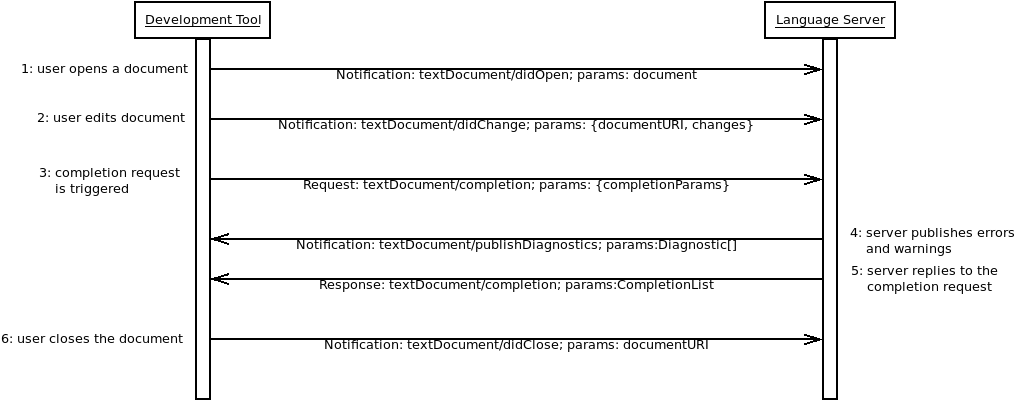
\includegraphics[width=\textwidth]{lsp.png}
\end{figure}

\begin{enumerate}
	\item \textbf{The user opens a file (refferred as a \textit{document})}: the tool notifies the server that a document is open ("textDocument/didOpen"), meaning that it is kept in the tool memory. The server will therefore save the language representation of the document in his memory.
	\item \textbf{The user edits the document}: the tool notifies the server about a change made by the user on the document ("textDocument/didChange"). The server updates the language representation of the document.
	\item \textbf{The tool execute the "Completion Request"}: the request ("textDocument/completion") is triggered by the aforementioned changes. The parameter, \textit{completionParams}, is essentially a JSON object with all the necessary information (documentURI, position, triggerKind) that the server needs to compute the response. Note that this call is \textit{asynchronous}: the tool can send other notifications or request while waiting for the completion response, same for the language server.
	\item \textbf{The server publishes errors and warnings}: after the change notification, the server computes and notifies the tool with a list of eventual errors and warnings in the code ("textDocument/publishDiagnostics"). The parameters of this notification contains all the necessary information in order to permit the tool flags errors and warnings.
	\item \textbf{The server replies to the "Completion Request"}: the server after computing a list of possible completion items, replies to the completion request made before by the tool. The latter lists the items received in order to let the user decide which suites the best.
	\item \textbf{The user closes the document}: the tool notifies the server when the user closes the document, which cease to exist in the tool memory. The server erases all the information regarding the aforementioned document. 
\end{enumerate}

All the data types illustrated are language agnostic, meaning that can be applied to all the programming languages. This is due to the protocol simplicity: it is more simple to standardize a document URI or a position inside a it, that standardizing an abstract syntax tree and compiler symbol across different programming languages.\\The aforementioned simplicity is shown in the following JSON-RPC objects that refers to the completion request and response:\\
\textbf{Request}:
\begin{lstlisting}[language=json]
{
	"jsonrpc": "2.0",
	"id" : 1,
	"method": "textDocument/completion",
	"params": {
		"textDocument": {
			"uri": "file:///home/user/Desktop/client.ol"
		},
		"position": {
			"line": 3,
			"character": 7
		},
		"context": {
			"triggerKind": 1
		}
	}
}
\end{lstlisting}
\textbf{Response}:
\begin{lstlisting}[language=json]
{
	"jsonrpc": "2.0",
	"id": 1,
	"result": {
	"isIncomplete": false,
		"items": {
			"label": "println@Console",
			"kind": 2,
			"insertText": "println@Console(  )(  )",
			"insertTextFormat": 2
		}
	}
}
\end{lstlisting}

A language server in order to work with LSP does not need to implement all the features. LSP provide \textbf{capabilities}. A capability groups a set of language features. The protocol permits the server to notify the tool which capabilities supports, therefore the tool adapts itself in order to send notifications and requests of the capabilities supported.
\chapter{Analysis of the problem}
In this chapter I will identify the requirements, gathered during the analysis of the Language Server Protocol and over a series of meetings with the supervisor.
\section{Language Server Protocol features}
LSP supports six key feature which are:
\begin{enumerate}
	\item \textbf{Code completion}: feature that speeds up the process of coding applications by reducing typos and other common mistakes;
	\item \textbf{Hover information}: feature that shows information, like the type signature, when the user moves the pointer over an element (such as a function definition);
	\item \textbf{Jump to definition}: feature that shows the definition of a selected symbol;
	\item \textbf{Workspace symbols}: displays all the symbols of the workspace, in order to help the user search for elements inside the workspace (such as classes, variables, methods, etc.);
	\item \textbf{Find references}: given a symbol, this features lists all the project wide references;
	\item \textbf{Diagnostics}: the tool flags syntax errors, warnings together with a description.
\end{enumerate}
The protocol supports many other features that are all linked to the above listed. The requirements elicitation phase was based on these main ones.
\section{Functional Requirements}
Functional requirements are statements of services the system should provide, particularly how it should react to particular inputs \cite{Som11}. From the features analyzed in the previous section, we extracted the following functional requirements, listed in ascending order of importance.
\begin{table}[H]
	\caption{Functional Requirements}
	\begin{tabularx}{\textwidth}{c|X}
		\hline
		\textbf{Functional r. No.} & \textbf{Description}\\
		\hline\hline
		FR 1 & The server must provide information of eventual programming errors and warnings every time a document is opened/modified.\\\hline
		FR 2 & Every time the user starts typing an operation name, the server returns a list of possible completion items that consists of the full operation name and the output port.\\\hline
		FR 3 & Every time the user starts typing a reserved word, the server provides a list of possible completion items.\\\hline
		FR 4 & Every time a document is opened/modified/closed, the server saves/updates/deletes the information in his memory like the text, URI and a data structure containing all the information regarding the Jolie program (an abstract syntax tree of the \textit{behavior} and data regarding the \textit{deployment}).\\\hline
		FR 5 & The server provides the type signature to the client every time the latter sends an hover request.\\\hline
		FR 6 & The server computes and sends the operation definition every time it receives a definition. request\\\hline
		FR 7 & The server provides a list or hierarchy of symbols of a specific document requested by the client.\\\hline
		FR 8 & Information regarding the workspace are sent to the client and updated every time the client requests them (workspace symbols for example).\\\hline
		FR 9 & The server resolves project wide references of a given symbol.\\\hline 
	\end{tabularx}
\end{table}

\section{Non-functional requirements}
Non-functional requirements are requirements that are not directly concerned with the specific services delivered by the system to its users. They may relate to emergent system properties such as reliability, response time, and store occupancy. Alternatively, they may define constraints on the system implementation such as the capabilities of I/O devices or the data representations used in interfaces with other systems \cite{Som11}.\\ Regarding the aforementioned non-functional requirements, the response time is critical for the project, as the server should be able to respond to the client as soon as possible. Nonetheless, this kind of calculations (such as code completion) are not computationally heavy.\\Other non-functional requirements, are listed below.
\subsection{Complying with the Language Server Protocol specification}
The Language Server Protocol defines a common language, between a tool and a language server. As a consequence, the latter must be able to recognize different requests received from the client and send back proper responses that the client is able to interpret and compute.\\Following an example: the request-response method \verb|initialize|, that provides the server client's capabilities and it expects a response with the server capabilities, has the following type:\\\textbf{Request type}
\begin{lstlisting}[language=javascript]
interface InitializeParams {
	processId: number | null;
	rootPath?: string | null;
	rootUri: DocumentUri | null;
	initializationOptions?: any;
	capabilities: ClientCapabilities;
	trace?: 'off' | 'messages' | 'verbose';
	workspaceFolders?: WorkspaceFolder[] | null;
}
\end{lstlisting}
\textbf{Response type}
\begin{lstlisting}[language=javascript]
interface InitializeResult {
	/**
	 * The capabilities the language server provides.
	 */
	capabilities: ServerCapabilities;
}
\end{lstlisting}
\subsubsection{JSON-RPC 2.0 Protocol}
Regarding the communication protocol, LSP supports a custom version of the JSON-RPC 2.0 protocol, as mentioned in \hyperref[sec:JolieLSP]{Chapter 2}. A message is characterized by an header part, which can contain up to two headers (Content-Length, which is mandatory, and Content-Type) and a content part, with the actual message represented with the JSON-RPC notation.\\Jolie supports JSON-RPC, but it runs over HTTP, therefore Jolie's JSON-RPC will expect HTTP headers before the Content-Length and Content-Type. As a consequence, Jolie's JSON-RPC protocol must be extended in order to make it compatible with LSP messages.
\subsection{Distributed}
The server must be adapted to the LSP, in order to make it works with different tools that uses the protocol concerned. Therefore, it must be \textbf{editor-agnostic} and it should be designed and implemented in order to be deployed both locally and in a different machine with respect to the clients, so it can interact with different tools at the same time. Consequently the best communication channel to use is the socket.
\subsection{Modular}
Not every language server can support all features defined by the protocol. LSP therefore provides, the previous mentioned, \textbf{capabilities}, as stated in \hyperref[sec:JolieLSP]{Chapter 2}. A capability groups a set of language features. A development tool and the language server announce their supported features using capabilities. For instance, the server announces that it can handle the \verb|textDocument/hover| request, but it might not support the \verb|textDocument/references| request. Similarly, a development tool announces its ability to provide \verb|textDocument/didChange| notification when a document is modified, so that a server can compute textual edits to format the edited document.\\On account of this, the server must be designed in order to easily add new capabilities or improve the existing ones. After implementing a new feature, the programmer just need to modify the server capabilities thus the client can start sending requests regarding the newly activated capability.

\begin{table}[H]
	\caption{Non-Functional Requirements}
	\begin{tabularx}{\textwidth}{c|X}
		\hline
		\textbf{Non-functional r. No.} & \textbf{Description}\\
		\hline\hline
		NFR 1 & The server must support the LSP's JSON-RPC protocol.\\\hline
		NFR 2 & The server must be designed to be modular.\\\hline
		NFR 3 & The server must be able to respond to a client request as soon as possible.\\\hline
		NFR 4 & The server must work both when deployed in a different machine and when deployed in a local machine, with respect of the client location. As a consequence, it has to support the socket channel of communication.\\\hline
		NFR 5 & The server if distributed, must be able to handle more clients sending multiple requests at the same time.\\\hline
	\end{tabularx}
\end{table}

\chapter{Design of the system}
\section{Architecture}
\subsection{Modules, interfaces, communication}
\section{What needs to be implemented}

\chapter{Implementation}
\label{sec:impl}
\section{Choosing a language: Jolie (why)}

\section{Implementation details}
\subsection{Complying with LSP's JSON-RPC protocol}
% TODO rivedere testo, far capire che c'� stato un problema di compatibilit� tra i protocolli
% e come si � risolto
The JSON-RPC 2.0 is a remote procedure call protocol that uses the JSON, a lightweight data-interchange format which is language independent. As stated in \hyperref[sec:JolieLSP]{Chapter 2}, an LSP message supports only two headers (\textit{Content-Lenghth} and \textit{Content-Type}), while the Jolie protocol runs over HTTP. This incompatibility led to a complex rework on the aforementioned Jolie protocol in order to meet the FR 1.\\ Further details can be read in \hyperref[sec:impl]{Chapter 5}.
\chapter{Validation}
\section{Met requirements (screenshots)}
\section{Unmet requirements}

\chapter{Conclusions: review, what needs to be done}

%% Fine dei capitoli normali, inizio dei capitoli-appendice (opzionali)
\appendix

\part{Appendici}

\chapter{Altro capitolo}

%% Parte conclusiva del documento; tipicamente per riassunto, bibliografia e/o indice analitico.
\backmatter

%% Riassunto (opzionale)
\summary

%% Bibliografia (opzionale)
\bibliographystyle{plain_\languagename}%% Carica l'omonimo file .bst, dove \languagename � la lingua attiva.
%% Nel caso in cui si usi un file .bib (consigliato)
\bibliography{thud}
%% Nel caso di bibliografia manuale, usare l'environment thebibliography.

%% Per l'indice analitico, usare il pacchetto makeidx (o analogo).

\end{document}

--- Istruzioni per l'aggiunta di nuove lingue ---
Per ogni nuova lingua utilizzata aggiungere nel preambolo il seguente spezzone:
    \addto\captionsitalian{%
        \def\abstractname{Sommario}%
        \def\acknowledgementsname{Ringraziamenti}%
        \def\authorcontactsname{Contatti dell'autore}%
        \def\candidatename{Candidato}%
        \def\chairname{Direttore}%
        \def\conclusionsname{Conclusioni}%
        \def\cosupervisorname{Co-relatore}%
        \def\cosupervisorsname{Co-relatori}%
        \def\cyclename{Ciclo}%
        \def\datename{Anno accademico}%
        \def\indexname{Indice analitico}%
        \def\institutecontactsname{Contatti dell'Istituto}%
        \def\introductionname{Introduzione}%
        \def\prefacename{Prefazione}%
        \def\reviewername{Controrelatore}%
        \def\reviewersname{Controrelatori}%
        %% Anno accademico
        \def\shortdatename{A.A.}%
        \def\summaryname{Riassunto}%
        \def\supervisorname{Relatore}%
        \def\supervisorsname{Relatori}%
        \def\thesisname{Tesi di \expandafter\ifcase\csname thud@target\endcsname Laurea\or Laurea Magistrale\or Dottorato\fi}%
        \def\tutorname{Tutor aziendale%
        \def\tutorsname{Tutor aziendali}%
    }
sostituendo a "italian" (nella 1a riga) il nome della lingua e traducendo le varie voci.
